\chapter{Δομή \& Οργάνωση Συστήματος}
Σε αυτό το κεφάλαιο, περιγράφονται λεπτομερώς οι λειτουργικές και μη-λειτουργικές απαιτήσεις του συστήματος διαχείρισης εκκίνησης υπολογιστών μέσω δικτύου. Επίσης, αναλύονται τα δύο είδη χρηστών που έχουν πρόσβαση στο σύστημα και οι δυνατότητες που παρέχονται από τη διαδικτυακή εφαρμογή του συστήματος. Ακόμα, γίνεται ανάλυση του σχήματος της βάσης δεδομένων και επεξήγηση αρχείων του κώδικα, ο οποίος συντέλεσε στη δημιουργία του πληροφοριακού συστήματος.

\section{Ανάλυση Συστήματος}
Για την επίτευξη της ορθής ανάλυσης και σχεδίασης του συστήματος, είναι απαραίτητη η κατανόηση των λειτουργιών του και των δυνατοτήτων που προσφέρει στους χρήστες του. Οι χρήστες είναι είτε γενικοί διαχειριστές του συστήματος, είτε διαχειριστές συγκεκριμένων εργαστηρίων.

Οι γενικοί διαχειριστές του συστήματος, έχουν τη δυνατότητα να προσθέτουν, να αφαιρούν και να επεξεργάζονται στοιχεία υπολογιστών, οι οποίοι δύναται να εκκινηθούν δικτυακά, με μενού επιλογής λειτουργικού συστήματος παρεχόμενο από το σύστημα. Μπορούν ακόμα να προσθέτουν και να διαχειρίζονται εργαστήρια στα οποία βρίσκονται οι υπολογιστές. Μια ακόμη ενέργεια στην οποία μπορούν να προβούν οι γενικοί διαχειριστές, είναι να τοποθετούν τους υπολογιστές σε ομάδες, οι οποίες καθορίζουν τα μενού λειτουργικών συστημάτων που θα παρέχονται από το σύστημα, ανάλογα με την τρέχουσα ημερομηνία / ώρα. Τέλος, οι γενικοί διαχειριστές ορίζουν τα διαθέσιμα λειτουργικά συστήματα, φτιάχνουν μενού εκκίνησης με χρήση των ορισμένων λειτουργικών συστημάτων και ρυθμίζουν τις ημερομηνίες / ώρες στις οποίες το σύστημα θα παρέχει τα μενού λειτουργικών συστημάτων στις ομάδες υπολογιστών.

Οι διαχειριστές εργαστηρίων, μπορούν να πραγματοποιούν τι ίδιες ενέργειες με τους γενικούς διαχειριστές, αλλά μόνο για τα εργαστήρια που τους έχουν ανατεθεί. Μπορούν δηλαδή να διαχειρίζονται τους υπολογιστές, τις ομάδες υπολογιστών και τα μενού εκκίνησης των ομάδων, που βρίσκονται στα εργαστήρια για τα οποία έχουν λάβει δικαίωμα διαχείρισης από τους γενικούς διαχειριστές.
 
\section{Ανάλυση Απαιτήσεων}

\subsection{Λειτουργικές Προδιαγραφές}
Η διαδικτυακή εφαρμογή που υλοποιήθηκε, δίνει τη δυνατότητα στον χρήστη να διαχειρίζεται τα μενού λειτουργικών συστημάτων κατά τη δικτυακή εκκίνηση ομάδων υπολογιστών.

\subsection{Μη-Λειτουργικές Προδιαγραφές}
Η διαδικτυακή εφαρμογή έχει υλοποιηθεί ως ένα web interface που επικοινωνεί με τη βάση δεδομένων μέσω ενός CRUD (Create - Read - Update - Delete) API, με χρήση του CodeIgniter PHP Framework.

\section{Περιπτώσεις Χρήσης}
Στους πίνακες που ακολουθούν παρουσιάζονται οι περιπτώσεις χρήσης της πλατφόρμας.

\FloatBarrier
\subsection{Βασικές Λειτουργίες Χρηστών}

%
% Εγγραφή χρήστη στο σύστημα
%
\begin{longtable}{|p{0.14\linewidth}|p{0.76\linewidth}|}
	\caption{Περίπτωση Χρήσης: Εγγραφή χρήστη στο σύστημα} \label{tab:use-case-signup} \\ \hline \endfirsthead
	\caption[{}]{Περίπτωση Χρήσης: Εγγραφή χρήστη στο σύστημα (συνέχεια)} \\ \endhead \endfoot
	Περιγραφή: & Ο τρόπος με τον οποίο εγγράφονται οι χρήστες στην πλατφόρμα \\ \hline
	Χειριστές: & Ανώνυμος Χρήστης \\ \hline
	Προϋποθέσεις: & Οι εγγραφές χρηστών στην πλατφόρμα πρέπει να είναι ενεργοποιημένες \\ \hline
	Βασική ροή: &
	\begin{enumerate}
		\vspace{-1cm}
		\addtolength{\itemindent}{-0.4cm}
		\item Ο χρήστης συμπληρώνει τα στοιχεία του στη σελίδα εγγραφής
		\item Επιβεβαιώνεται η επιτυχής εισαγωγή των στοιχείων και γίνεται επαλήθευσή τους από client-side και server-side validators για την εξακρίβωση τύπου και πλήθους δεδομένων
		\item Η εγγραφή του χρήστη στο σύστημα ολοκληρώνεται, ο χρήστης μεταφέρεται στη σελίδα σύνδεσης και παράλληλα λαμβάνει email με σύνδεσμο επιβεβαίωσης της διεύθυνσης email του
		\item Η χρονοσφραγίδα επιτυχούς εγγραφής χρήστη στο σύστημα καταγράφεται στο αρχείο συμβάντων
		\vspace{-0.7cm}
	\end{enumerate} \\ \hline
	Εναλλακτικό σενάριο: & O χρήστης εισάγει εσφαλμένα στοιχεία, η πλατφόρμα απορρίπτει τη σύνδεση, εμφανίζει μήνυμα σφάλματος και ζητά από τον χρήστη να δοκιμάσει ξανά να εισαγάγει τα σωστά στοιχεία \\ \hline
\end{longtable}

\textbf{Σημείωση:} Στον πίνακα \ref{tab:use-case-signup} περιγράφεται η περίπτωση χρήσης εγγραφής νέου χρήστη στην πλατφόρμα. Κατά την πρώτη περιήγηση στην αρχική σελίδα της εφαρμογής, μετά την εγκατάσταση της και όταν δεν υπάρχει εγγεγραμμένος Γενικός Διαχειριστής Πλατφόρμας, θα ξεκινήσει η διαδικασία εγγραφής Γενικού Διαχειριστή Πλατφόρμας, ανεξάρτητα από το αν οι εγγραφές χρηστών είναι ενεργοποιημένες. Οι επόμενοι χρήστες που θα εγγραφούν δε παίρνουν αυτόματα αυτό το ρόλο.

%
% Σύνδεση στο σύστημα
%
\begin{longtable}{|p{0.14\linewidth}|p{0.76\linewidth}|}
	\caption{Περίπτωση Χρήσης: Σύνδεση χρήστη στο σύστημα} \label{tab:use-case-login} \\ \hline \endfirsthead
	\caption[{}]{Περίπτωση Χρήσης: Σύνδεση χρήστη στο σύστημα (συνέχεια)} \\ \endhead \endfoot
	Περιγραφή: & Ο τρόπος με τον οποίο συνδέεται ο χρήστης στην πλατφόρμα \\ \hline
	Χειριστές: & Γενικός Διαχειριστής Πλατφόρμας, Διαχειριστής Εργαστηρίου \\ \hline
	Προϋποθέσεις: & Ο χρήστης πρέπει να είναι εγγεγραμμένος στην πλατφόρμα \\ \hline
	Βασική ροή: &
	\begin{enumerate}
		\vspace{-1cm}
		\addtolength{\itemindent}{-0.4cm}
		\item Ο χρήστης δεν έχει cookie αυθεντικοποίησης χρήστη της εφαρμογής στον περιηγητή ιστού του
		\item Ο χρήστης εισάγει το όνομα χρήστη και τον κωδικό πρόσβασης του λογαριασμού του
		\item Επιβεβαιώνεται η επιτυχής εισαγωγή των στοιχείων σύνδεσης
		\item O χρήστης συνδέεται στο σύστημα και αποθηκεύεται cookie αυθεντικοποίησης χρήστη της εφαρμογής στον περιηγητή ιστού του
		\item Η χρονοσφραγίδα επιτυχούς σύνδεσης του χρήστη καταγράφεται στο αρχείο συμβάντων
		\vspace{-0.7cm}
	\end{enumerate} \\ \hline
	Εναλλακτικό σενάριο: & O χρήστης εισάγει εσφαλμένα στοιχεία, η πλατφόρμα απορρίπτει τη σύνδεση, εμφανίζει μήνυμα σφάλματος, καταγράφει την αποτυχία σύνδεσης και ζητά από τον χρήστη να δοκιμάσει ξανά να εισαγάγει τα σωστά στοιχεία \\ \hline
\end{longtable}

%
% Επανέκδοση κωδικού χρήστη
%
\begin{longtable}{|p{0.14\linewidth}|p{0.76\linewidth}|}
	\caption{Περίπτωση Χρήσης: Επανέκδοση κωδικού χρήστη} \label{tab:use-case-forgot-password} \\ \hline \endfirsthead
	\caption[{}]{Περίπτωση Χρήσης: Επανέκδοση κωδικού χρήστη (συνέχεια)} \\ \endhead \endfoot
	Περιγραφή: & Ο τρόπος με τον οποίο ο χρήστης δημιουργεί νέο κωδικό για τον λογαριασμό του σε περίπτωση που ξεχάσει τον παλιό \\ \hline
	Χειριστές: & Γενικός Διαχειριστής Πλατφόρμας, Διαχειριστής Εργαστηρίου \\ \hline
	Προϋποθέσεις: & Καμία \\ \hline
	Βασική ροή: &
	\begin{enumerate}
		\vspace{-1cm}
		\addtolength{\itemindent}{-0.4cm}
		\item Ο χρήστης έχει ξεχάσει τον κωδικό του λογαριασμού του
		\item Ο χρήστης περιηγείται στο σημείο επανέκδοσης κωδικού πρόσβασης
		\item Εισάγει το όνομα χρήστη ή το email του στη φόρμα
		\item Λαμβάνει στο email του έναν ειδικό σύνδεσμο επανέκδοσης του κωδικού του
		\item Ακολουθεί τον σύνδεσμο και εισάγει τον νέο κωδικού του λογαριασμού του
		\item Συνδέεται στην πλατφόρμα με χρήση του νέου κωδικού του
		\item Η χρονοσφραγίδα αλλαγής του κωδικού πρόσβασης του χρήστη καταγράφεται στο αρχείο συμβάντων
		\vspace{-0.7cm}
	\end{enumerate} \\ \hline
	Εναλλακτικό σενάριο: & Αν ο χρήστης εισάγει λάθος στοιχεία στο βήμα 3, δε θα λάβει το email επαναφοράς του κωδικού του \\ \hline
\end{longtable}

%
% Υπενθύμιση Ονόματος Χρήστη
%
\begin{longtable}{|p{0.14\linewidth}|p{0.76\linewidth}|}
	\caption{Περίπτωση Χρήσης: Υπενθύμιση Ονόματος Χρήστη} \label{tab:use-case-forgot-username} \\ \hline \endfirsthead
	\caption[{}]{Περίπτωση Χρήσης: Υπενθύμιση Ονόματος Χρήστη (συνέχεια)} \\ \endhead \endfoot
	Περιγραφή: & Ο τρόπος με τον οποίο ο χρήστης ζητά email υπενθύμισης για το όνομα χρήστη του λογαριασμού του \\ \hline
	Χειριστές: & Γενικός Διαχειριστής Πλατφόρμας, Διαχειριστής Εργαστηρίου \\ \hline
	Προϋποθέσεις: & Καμία \\ \hline
	Βασική ροή: &
	\begin{enumerate}
		\vspace{-1cm}
		\addtolength{\itemindent}{-0.4cm}
		\item Ο χρήστης έχει ξεχάσει το όνομα χρήστη του λογαριασμού του
		\item Ο χρήστης περιηγείται στο σημείο υπενθύμισης ονόματος χρήστη
		\item Εισάγει το email του λογαριασμού του
		\item Λαμβάνει στο email του υπενθύμιση του ονόματος χρήστη του
		\item Η χρονοσφραγίδα αποστολής του μηνύματος υπενθύμισης του ονόματος χρήστη του χρήστη καταγράφεται στο αρχείο συμβάντων
		\vspace{-0.7cm}
	\end{enumerate} \\ \hline
	Εναλλακτικό σενάριο: & Αν ο χρήστης εισάγει λάθος email στο βήμα 3, δε θα λάβει το email υπενθύμισης του ονόματος χρήστη του \\ \hline
\end{longtable}

%
% Αποσύνδεση από το σύστημα
%
\begin{longtable}{|p{0.14\linewidth}|p{0.76\linewidth}|}
	\caption{Περίπτωση Χρήσης: Αποσύνδεση από το σύστημα} \label{tab:use-case-logout} \\ \hline \endfirsthead
	\caption[{}]{Περίπτωση Χρήσης: Αποσύνδεση από το σύστημα (συνέχεια)} \\ \endhead \endfoot
	Περιγραφή: & Ο τρόπος με τον οποίο ο χρήστης αποσυνδέεται από την πλατφόρμα \\ \hline
	Χειριστές: & Γενικός Διαχειριστής Πλατφόρμας, Διαχειριστής Εργαστηρίου \\ \hline
	Προϋποθέσεις: & Καμία \\ \hline
	Βασική ροή: &
	\begin{enumerate}
		\vspace{-1cm}
		\addtolength{\itemindent}{-0.4cm}
		\item Ο χρήστης επιλέγει το κουμπί της Αποσύνδεσης από το κεντρικό μενού
		\item Ο χρήστης αποσυνδέεται από το σύστημα και διαγράφεται το cookie αυθεντικοποίησης χρήστη της εφαρμογής από τον περιηγητή ιστού του
		\vspace{-0.7cm}
	\end{enumerate} \\ \hline
	Εναλλακτικό σενάριο: & \\ \hline
\end{longtable}

%
% Αλλαγή στοιχείων χρήστη
%
\begin{longtable}{|p{0.14\linewidth}|p{0.76\linewidth}|}
	\caption{Περίπτωση Χρήσης: Αλλαγή στοιχείων χρήστη} \label{tab:use-case-change-profile} \\ \hline \endfirsthead
	\caption[{}]{Περίπτωση Χρήσης: Αλλαγή στοιχείων χρήστη (συνέχεια)} \\ \endhead \endfoot
	Περιγραφή: & Ο τρόπος με τον οποίο ο χρήστης αλλάζει τα στοιχεία του προφίλ του \\ \hline
	Χειριστές: & Γενικός Διαχειριστής Πλατφόρμας, Διαχειριστής Εργαστηρίου \\ \hline
	Προϋποθέσεις: & Καμία \\ \hline
	Βασική ροή: &
	\begin{enumerate}
		\vspace{-1cm}
		\addtolength{\itemindent}{-0.4cm}
		\item Ο χρήστης περιηγείται στο προφίλ του από το κεντρικό μενού
		\item Επιλέγει την επεξεργασία προφίλ
		\item Αλλάζει τα στοιχεία που επιθυμεί (όνομα χρήστη, κωδικό πρόσβασης, email, τηλέφωνο)
		\item Επιλέγει την αποθήκευση αλλαγών
		\item Η χρονοσφραγίδα επιτυχούς αλλαγής των στοιχείων του χρήστη καταγράφεται στο αρχείο συμβάντων
		\vspace{-0.7cm}
	\end{enumerate} \\ \hline
	Εναλλακτικό σενάριο: &
	\begin{itemize}
		\vspace{-1cm}
		\addtolength{\itemindent}{-0.4cm}
		\item Αν τα νέα στοιχεία είναι εσφαλμένα, η πλατφόρμα απορρίπτει την αποθήκευσή τους, εμφανίζει μήνυμα σφάλματος και ζητά από τον χρήστη να δοκιμάσει ξανά να εισαγάγει έγκυρα στοιχεία
		\item Αν ο χρήστης είναι Γενικός Διαχειριστής Πλατφόρμας, μπορεί να περιηγηθεί στη σελίδα με τη λίστα χρηστών και από εκεί να επεξεργαστεί τα στοιχεία άλλων χρήστων και επιπρόσθετα να αλλάξει το ρόλο τους
		\vspace{-0.7cm}
	\end{itemize} \\ \hline
\end{longtable}

%
% Διαγραφή χρήστη από το σύστημα
%
\begin{longtable}{|p{0.14\linewidth}|p{0.76\linewidth}|}
	\caption{Περίπτωση Χρήσης: Διαγραφή χρήστη από το σύστημα} \label{tab:use-case-delete-user} \\ \hline \endfirsthead
	\caption[{}]{Περίπτωση Χρήσης: Διαγραφή χρήστη από το σύστημα (συνέχεια)} \\ \endhead \endfoot
	Περιγραφή: & Ο τρόπος με τον οποίο ο χρήστης αποσυνδέεται από την πλατφόρμα \\ \hline
	Χειριστές: & Γενικός Διαχειριστής Πλατφόρμας, Διαχειριστής Εργαστηρίου \\ \hline
	Προϋποθέσεις: & Καμία \\ \hline
	Βασική ροή: &
	\begin{enumerate}
		\vspace{-1cm}
		\addtolength{\itemindent}{-0.4cm}
		\item Ο χρήστης περιηγείται στο προφίλ του από το κεντρικό μενού
		\item Επιλέγει τη διαγραφή του χρήστη του από την πλατφόρμα
		\item Εμφανίζεται ένα αναδυόμενο παράθυρο στο οποίο ο χρήστης επιβεβαιώνει την οριστική διαγραφή του από την πλατφόρμα
		\item Ο χρήστης αποσυνδέεται και τα στοιχεία του διαγράφονται από την πλατφόρμα
		\item Η χρονοσφραγίδα διαγραφής του χρήστη καταγράφεται στο αρχείο συμβάντων
		\vspace{-0.7cm}
	\end{enumerate} \\ \hline
	Εναλλακτικό σενάριο: &
	\begin{itemize}
		\vspace{-1cm}
		\addtolength{\itemindent}{-0.4cm}
		\item Αν ο χρήστης δεν επιβεβαιώσει την οριστική διαγραφή του στο βήμα 3, τα στοιχεία του δε διαγράφονται και παραμένει συνδεδεμένος
		\item Αν ο χρήστης είναι Γενικός Διαχειριστής Πλατφόρμας, μπορεί να περιηγηθεί στη σελίδα με τη λίστα χρηστών και από εκεί να διαγράψει άλλους χρήστες
		\vspace{-0.7cm}
	\end{itemize} \\ \hline
\end{longtable}

\subsection{Διαχείριση Εργαστηρίων}

%
% Εισαγωγή εργαστηρίου στο σύστημα
%
\begin{longtable}{|p{0.14\linewidth}|p{0.76\linewidth}|}
	\caption{Περίπτωση Χρήσης: Εισαγωγή εργαστηρίου στο σύστημα} \label{tab:use-case-add-lab} \\ \hline \endfirsthead
	\caption[{}]{Περίπτωση Χρήσης: Εισαγωγή εργαστηρίου στο σύστημα (συνέχεια)} \\ \endhead \endfoot
	Περιγραφή: & Ο τρόπος με τον οποίο ο Γενικός Διαχειριστής προσθέτει ένα εργαστήριο το σύστημα \\ \hline
	Χειριστές: & Γενικός Διαχειριστής Πλατφόρμας \\ \hline
	Προϋποθέσεις: & Καμία \\ \hline
	Βασική ροή: &
	\begin{enumerate}
		\vspace{-1cm}
		\addtolength{\itemindent}{-0.4cm}
		\item Ο χρήστης περιηγείται στη σελίδα με τη λίστα των εργαστηρίων
		\item Επιλέγει την προσθήκη νέου εργαστηρίου
		\item Εισαγάγει τα στοιχεία του νέου εργαστηρίου (όνομα και προαιρετικά διεύθυνση ή/και τηλέφωνο)
		\item Επιλέγει την αποθήκευση αλλαγών
		\item Η χρονοσφραγίδα επιτυχούς εισαγωγής εργαστηρίου από τον χρήστη καταγράφεται στο αρχείο συμβάντων
		\vspace{-0.7cm}
	\end{enumerate} \\ \hline
	Εναλλακτικό σενάριο: & Αν ο χρήστης δεν αποθηκεύσει τις αλλαγές στο βήμα 4, το νέο εργαστήριο δε θα προστεθεί \\ \hline
\end{longtable}

%
% Διαγραφή εργαστηρίου από το σύστημα
%
\begin{longtable}{|p{0.14\linewidth}|p{0.76\linewidth}|}
	\caption{Περίπτωση Χρήσης: Διαγραφή εργαστηρίου από το σύστημα} \label{tab:use-case-delete-lab} \\ \hline \endfirsthead
	\caption[{}]{Περίπτωση Χρήσης: Διαγραφή εργαστηρίου από το σύστημα (συνέχεια)} \\ \endhead \endfoot
	Περιγραφή: & Ο τρόπος με τον οποίο ο Γενικός Διαχειριστής αφαιρεί ένα εργαστήριο από το σύστημα \\ \hline
	Χειριστές: & Γενικός Διαχειριστής Πλατφόρμας \\ \hline
	Προϋποθέσεις: & Το εργαστήριο πρέπει να έχει προστεθεί στο σύστημα \\ \hline
	Βασική ροή: &
	\begin{enumerate}
		\vspace{-1cm}
		\addtolength{\itemindent}{-0.4cm}
		\item Ο χρήστης περιηγείται στη σελίδα με τη λίστα των εργαστηρίων
		\item Επιλέγει το σύμβολο διαγραφής, δίπλα στα στοιχεία του εργαστηρίου που θέλει να διαγράψει
		\item Επιβεβαιώνει την οριστική διαγραφή του εργαστηρίου στο αναδυόμενο παράθυρο που εμφανίζεται
		\item Τα στοιχεία του εργαστηρίου διαγράφονται από την πλατφόρμα και οι υπολογιστές που του είχαν ανατεθεί μεταφέρονται στη λίστα αναμονής ανάθεσης σε εργαστήριο
		\item Η χρονοσφραγίδα επιτυχούς διαγραφής εργαστηρίου από τον χρήστη καταγράφεται στο αρχείο συμβάντων
		\vspace{-0.7cm}
	\end{enumerate} \\ \hline
	Εναλλακτικό σενάριο: & Αν ο χρήστης δεν επιβεβαιώσει τη διαγραφή του εργαστηρίου στο βήμα 3, τα στοιχεία του παραμένουν στην πλατφόρμα \\ \hline
\end{longtable}

%
% Επεξεργασία αναθέσεων Διαχειριστών Εργαστηρίων
%
\begin{longtable}{|p{0.14\linewidth}|p{0.76\linewidth}|}
	\caption{Περίπτωση Χρήσης: Επεξεργασία αναθέσεων Διαχειριστών Εργαστηρίων} \label{tab:use-case-edit-lab-admin} \\ \hline \endfirsthead
	\caption[{}]{Περίπτωση Χρήσης: Επεξεργασία αναθέσεων Διαχειριστών Εργαστηρίων (συνέχεια)} \\ \endhead \endfoot
	Περιγραφή: & Ο τρόπος με τον οποίο ο Γενικός Διαχειριστής Πλατφόρμας επεξεργάζεται τις αναθέσεις Διαχειριστών Εργαστηρίων \\ \hline
	Χειριστές: & Γενικός Διαχειριστής Πλατφόρμας \\ \hline
	Προϋποθέσεις: & Ο χρήστης προς ανάθεση πρέπει να έχει εγγραφεί στο σύστημα \\ \hline
	Βασική ροή: &
	\begin{enumerate}
		\vspace{-1cm}
		\addtolength{\itemindent}{-0.4cm}
		\item Ο χρήστης περιηγείται στη σελίδα με τη λίστα των εργαστηρίων
		\item Επιλέγει την επεξεργασία στοιχείων
		\item Επιλέγει τους Διαχειριστές Εργαστηρίου για κάθε εργαστήριο που θέλει να επεξεργαστεί
		\item Επιλέγει την αποθήκευση αλλαγών
		\item Η χρονοσφραγίδα επιτυχούς επεξεργασίας του κάθε εργαστηρίου από τον Γενικό Διαχειριστή Πλατφόρμας καταγράφεται στο αρχείο συμβάντων
		\vspace{-0.7cm}
	\end{enumerate} \\ \hline
	Εναλλακτικό σενάριο: &
	\begin{enumerate}
		\vspace{-1cm}
		\addtolength{\itemindent}{-0.4cm}
		\item Ο χρήστης περιηγείται στη σελίδα με τη λίστα χρηστών
		\item Επιλέγει την επεξεργασία στοιχείων
		\item Επιλέγει τα εργαστήρια στα οποία θέλει να είναι Διαχειριστές Εργαστηρίου σε όσους χρήστες θέλει να επεξεργαστεί
		\item Επιλέγει την αποθήκευση αλλαγών
		\item Η χρονοσφραγίδα επιτυχούς επεξεργασίας του κάθε χρήστη από τον Γενικό Διαχειριστή Πλατφόρμας καταγράφεται στο αρχείο συμβάντων
		\vspace{-0.7cm}
	\end{enumerate} \\ \hline
\end{longtable}

\subsection{Διαχείριση Ομάδων Υπολογιστών}

%
% Δημιουργία ομάδας υπολογιστών
%
\begin{longtable}{|p{0.14\linewidth}|p{0.76\linewidth}|}
	\caption{Περίπτωση Χρήσης: Δημιουργία ομάδας υπολογιστών} \label{tab:use-case-add-group} \\ \hline \endfirsthead
	\caption[{}]{Περίπτωση Χρήσης: Δημιουργία ομάδας υπολογιστών (συνέχεια)} \\ \endhead \endfoot
	Περιγραφή: & Ο τρόπος με τον οποίο δημιουργείται μια ομάδα υπολογιστών \\ \hline
	Χειριστές: & Γενικός Διαχειριστής Πλατφόρμας, Διαχειριστής Εργαστηρίου \\ \hline
	Προϋποθέσεις: & Καμία \\ \hline
	Βασική ροή: &
	\begin{enumerate}
		\vspace{-1cm}
		\addtolength{\itemindent}{-0.4cm}
		\item Ο χρήστης περιηγείται στη σελίδα με τη λίστα των ομάδων υπολογιστών
		\item Επιλέγει την προσθήκη νέας εγγραφής
		\item Εισαγάγει τα στοιχεία της νέας ομάδας υπολογιστών (όνομα, διεύθυνση και prefix εικόνων λειτουργικών συστημάτων)
		\item Επιλέγει την αποθήκευση αλλαγών
		\item Η χρονοσφραγίδα επιτυχούς δημιουργίας ομάδας υπολογιστών από τον χρήστη καταγράφεται στο αρχείο συμβάντων
		\vspace{-0.7cm}
	\end{enumerate} \\ \hline
	Εναλλακτικό σενάριο: & Αν ο χρήστης δεν αποθηκεύσει τις αλλαγές στο βήμα 4, η νέα ομάδας υπολογιστών δε θα προστεθεί \\ \hline
\end{longtable}

%
% Διαγραφή ομάδας υπολογιστών
%
\begin{longtable}{|p{0.14\linewidth}|p{0.76\linewidth}|}
	\caption{Περίπτωση Χρήσης: Διαγραφή ομάδας υπολογιστών} \label{tab:use-case-delete-group} \\ \hline \endfirsthead
	\caption[{}]{Περίπτωση Χρήσης: Διαγραφή ομάδας υπολογιστών (συνέχεια)} \\ \endhead \endfoot
	Περιγραφή: & Ο τρόπος με τον οποίο διαγράφεται μια ομάδα υπολογιστών \\ \hline
	Χειριστές: & Γενικός Διαχειριστής Πλατφόρμας, Διαχειριστής Εργαστηρίου \\ \hline
	Προϋποθέσεις: & Η ομάδα υπολογιστών πρέπει να έχει προστεθεί στο σύστημα \\ \hline
	Βασική ροή: &
	\begin{enumerate}
		\vspace{-1cm}
		\addtolength{\itemindent}{-0.4cm}
		\item Ο χρήστης περιηγείται στη σελίδα με τη λίστα των ομάδων υπολογιστών
		\item Επιλέγει το σύμβολο διαγραφής, δίπλα στα στοιχεία της ομάδας υπολογιστών που θέλει να διαγράψει
		\item Επιβεβαιώνει τη διαγραφή στο αναδυόμενο παράθυρο που θα εμφανιστεί
		\item Τα στοιχεία της ομάδας υπολογιστών διαγράφονται από την πλατφόρμα
		\item Η χρονοσφραγίδα επιτυχούς διαγραφής ομάδας υπολογιστών από τον χρήστη καταγράφεται στο αρχείο συμβάντων
		\vspace{-0.7cm}
	\end{enumerate} \\ \hline
	Εναλλακτικό σενάριο: & Αν ο χρήστης δεν επιβεβαιώσει τη διαγραφή της ομάδας υπολογιστών στο βήμα 3, τα στοιχεία της παραμένουν στην πλατφόρμα \\ \hline
\end{longtable}

\subsection{Διαχείριση Υπολογιστών}

%
% Εισαγωγή υπολογιστή στο σύστημα
%
\begin{longtable}{|p{0.14\linewidth}|p{0.76\linewidth}|}
	\caption{Περίπτωση Χρήσης: Εισαγωγή υπολογιστή στο σύστημα} \label{tab:use-case-add-computer} \\ \hline \endfirsthead
	\caption[{}]{Περίπτωση Χρήσης: Εισαγωγή υπολογιστή στο σύστημα (συνέχεια)} \\ \endhead \endfoot
	Περιγραφή: & Ο τρόπος με τον οποίο ο διαχειριστής προσθέτει έναν υπολογιστή στο σύστημα \\ \hline
	Χειριστές: & Γενικός Διαχειριστής Πλατφόρμας, Διαχειριστής Εργαστηρίου \\ \hline
	Προϋποθέσεις: & Πρέπει να έχει ρυθμιστεί ο DHCP server του εργαστηρίου στο οποίο βρίσκεται ο υπολογιστής, ώστε να παρέχει τη διεύθυνση του συστήματος για δικτυακή εκκίνηση των υπολογιστών \\ \hline
	Βασική ροή: &
	\begin{enumerate}
		\vspace{-1cm}
		\addtolength{\itemindent}{-0.4cm}
		\item Ο υπολογιστής εκκινείται και τα στοιχεία του υπολογιστή (το UUID της μητρικής πλακέτας και η φυσική διεύθυνση MAC της διεπαφής δικτύου) καταγράφονται στο σύστημα και εμφανίζονται στην οθόνη του υπολογιστή
		\item Ο χρήστης βλέπει την νέα εγγραφή στο σύστημα, στην οθόνη με τους υπολογιστές που δεν έχουν ανατεθεί σε εργαστήριο. Μπορεί να επαληθεύσει την ταυτότητα του υπολογιστή συγκρίνοντας τα στοιχεία που βλέπει στο σύστημα με αυτά που εμφανίζονται στην οθόνη του υπολογιστή
		\item Ο χρήστης συμπληρώνει τα απαραίτητα στοιχεία για τον υπολογιστή (όνομα και προαιρετικά σημειώσεις για τον υπολογιστή, το εργαστήριο στο οποίο βρίσκεται, τις ομάδες υπολογιστών στις οποίες ανήκει)
		\item Ο υπολογιστής είναι έτοιμος να εκκινηθεί μέσω του συστήματος και μπορούν να διαχειριστούν τα στοιχεία του, τόσο οι γενικοί διαχειριστές του συστήματος, όσο και οι διαχειριστές του εργαστηρίου στο οποίο ανήκει
		\vspace{-0.7cm}
	\end{enumerate} \\ \hline
	Εναλλακτικό σενάριο: & Ο χρήστης γνωρίζει εκ των προτέρων τα στοιχεία του υπολογιστή και τα προσθέτει στο σύστημα \\ \hline
\end{longtable}

%
% Ανάθεση υπολογιστή σε εργαστήριο
%
\begin{longtable}{|p{0.14\linewidth}|p{0.76\linewidth}|}
	\caption{Περίπτωση Χρήσης: Ανάθεση υπολογιστή σε εργαστήριο} \label{tab:use-case-add-computer-to-lab} \\ \hline \endfirsthead
	\caption[{}]{Περίπτωση Χρήσης: Ανάθεση υπολογιστή σε εργαστήριο (συνέχεια)} \\ \endhead \endfoot
	Περιγραφή: & Ο τρόπος με τον οποίο ένας υπολογιστής ανατίθεται σε ένα εργαστήριο \\ \hline
	Χειριστές: & Γενικός Διαχειριστής Πλατφόρμας, Διαχειριστής Εργαστηρίου \\ \hline
	Προϋποθέσεις: &
	\begin{itemize}
		\vspace{-1cm}
		\addtolength{\itemindent}{-0.4cm}
		\item Ο υπολογιστής πρέπει να έχει προστεθεί στο σύστημα και να μην έχει ανατεθεί ήδη σε κάποιο άλλο εργαστήριο
		\item Αν ο χρήστης είναι Διαχειριστής Εργαστηρίου, στο βήμα 2 μπορεί να αναθέσει υπολογιστή μόνο σε εργαστήριο το οποίο διαχειρίζεται ο ίδιος. Αν είναι Γενικός Διαχειριστής της πλατφόρμας μπορεί να αναθέσει τον υπολογιστή σε οποιοδήποτε εργαστήριο.
		\vspace{-0.7cm}
	\end{itemize} \\ \hline
	Βασική ροή: &
	\begin{enumerate}
		\vspace{-1cm}
		\addtolength{\itemindent}{-0.4cm}
		\item Ο χρήστης εντοπίζει τον υπολογιστή στη λίστα αναμονής ανάθεσης σε εργαστήριο
		\item Επιλέγει το εργαστήριο στο οποίο θα ανατεθεί ο υπολογιστής
		\item Επιλέγει την αποθήκευση αλλαγών
		\item Η χρονοσφραγίδα επιτυχούς ανάθεσης του υπολογιστή στο εργαστήριο από τον χρήστη καταγράφεται στο αρχείο συμβάντων
		\vspace{-0.7cm}
	\end{enumerate} \\ \hline
	Εναλλακτικό σενάριο: & Αν ο χρήστης δεν αποθηκεύσει τις αλλαγές στο βήμα 3, ο υπολογιστής δε θα ανατεθεί στο εργαστήριο \\ \hline
\end{longtable}

%
% Αφαίρεση υπολογιστή από εργαστήριο
%
\begin{longtable}{|p{0.14\linewidth}|p{0.76\linewidth}|}
	\caption{Περίπτωση Χρήσης: Αφαίρεση υπολογιστή από εργαστήριο} \label{tab:use-case-delete-computer-from-lab} \\ \hline \endfirsthead
	\caption[{}]{Περίπτωση Χρήσης: Αφαίρεση υπολογιστή από εργαστήριο (συνέχεια)} \\ \endhead \endfoot
	Περιγραφή: & Ο τρόπος με τον οποίο ένας υπολογιστής διαγράφεται από ένα εργαστήριο \\ \hline
	Χειριστές: & Γενικός Διαχειριστής Πλατφόρμας, Διαχειριστής Εργαστηρίου \\ \hline
	Προϋποθέσεις: &
	\begin{itemize}
		\vspace{-1cm}
		\addtolength{\itemindent}{-0.4cm}
		\item Ο υπολογιστής πρέπει να έχει προστεθεί στο εργαστήριο
		\item Αν ο χρήστης είναι Διαχειριστής Εργαστηρίου, στο βήμα 1 μπορεί να αφαιρέσει υπολογιστές μόνο από εργαστήριο το οποίο διαχειρίζεται ο ίδιος. Αν είναι Γενικός Διαχειριστής της πλατφόρμας δεν υπάρχει τέτοιος περιορισμός.
		\vspace{-0.7cm}
	\end{itemize} \\ \hline
	Βασική ροή: &
	\begin{enumerate}
		\vspace{-1cm}
		\addtolength{\itemindent}{-0.4cm}
		\item Ο χρήστης εντοπίζει τον υπολογιστή στη λίστα υπολογιστών του εργαστηρίου στο οποίο έχει ανατεθεί
		\item Επιλέγει το σύμβολο διαγραφής, δίπλα στα στοιχεία του υπολογιστή που θέλει να αφαιρέσει
		\item Επιβεβαιώνει την αφαίρεση του υπολογιστή από το εργαστήριο στο αναδυόμενο παράθυρο που εμφανίζεται
		\item Ο υπολογιστής αφαιρείται από το εργαστήριο και μεταφέρεται στη λίστα αναμονής ανάθεσης σε εργαστήριο
		\item Η χρονοσφραγίδα επιτυχούς αφαίρεσης του υπολογιστή από το εργαστήριο από τον χρήστη καταγράφεται στο αρχείο συμβάντων
		\vspace{-0.7cm}
	\end{enumerate} \\ \hline
	Εναλλακτικό σενάριο: & Αν ο χρήστης δεν επιβεβαιώσει την αφαίρεση του υπολογιστή στο βήμα 3, ο υπολογιστής παραμένει στο εργαστήριο \\ \hline
\end{longtable}

%
% Επεξεργασία στοιχείων υπολογιστή
%
\begin{longtable}{|p{0.14\linewidth}|p{0.76\linewidth}|}
	\caption{Περίπτωση Χρήσης: Επεξεργασία στοιχείων υπολογιστή} \label{tab:use-case-edit-computer} \\ \hline \endfirsthead
	\caption[{}]{Περίπτωση Χρήσης: Επεξεργασία στοιχείων υπολογιστή (συνέχεια)} \\ \endhead \endfoot
	Περιγραφή: & Ο τρόπος με τον οποίο γίνεται επεξεργασία των στοιχείων ενός υπολογιστή \\ \hline
	Χειριστές: & Γενικός Διαχειριστής Πλατφόρμας, Διαχειριστής Εργαστηρίου \\ \hline
	Προϋποθέσεις: &
	\begin{itemize}
		\vspace{-1cm}
		\addtolength{\itemindent}{-0.4cm}
		\item Ο υπολογιστής πρέπει να έχει προστεθεί στο σύστημα
		\item Αν ο χρήστης είναι Διαχειριστής Εργαστηρίου, στο βήμα 1 μπορεί να επεξεργαστεί τα στοιχεία μόνο υπολογιστών που έχουν ανατεθεί σε εργαστήριο το οποίο διαχειρίζεται ο ίδιος. Αν είναι Γενικός Διαχειριστής της πλατφόρμας δεν υπάρχει τέτοιος περιορισμός.
		\vspace{-0.7cm}
	\end{itemize} \\ \hline
	Βασική ροή: &
	\begin{enumerate}
		\vspace{-1cm}
		\addtolength{\itemindent}{-0.4cm}
		\item Ο χρήστης εντοπίζει τον υπολογιστή στη λίστα υπολογιστών του εργαστηρίου στο οποίο έχει ανατεθεί, ή στη λίστα αναμονής ανάθεσης σε εργαστήριο
		\item Επιλέγει την επεξεργασία στοιχείων
		\item Πραγματοποιεί αλλαγές στα στοιχεία του υπολογιστή (όνομα, MAC, UUID, σημειώσεις, εργαστήριο, ομάδες υπολογιστών στις οποίες ανήκει)
		\item Επιλέγει την αποθήκευση αλλαγών
		\item Η χρονοσφραγίδα επιτυχούς επεξεργασίας των στοιχείων του υπολογιστή από τον χρήστη καταγράφεται στο αρχείο συμβάντων
		\vspace{-0.7cm}
	\end{enumerate} \\ \hline
	Εναλλακτικό σενάριο: & Αν ο χρήστης δεν αποθηκεύσει τις αλλαγές στο βήμα 4, τα στοιχεία του υπολογιστή παραμένουν ως έχουν \\ \hline
\end{longtable}

%
% Διαγραφή υπολογιστή από το σύστημα
%
\begin{longtable}{|p{0.14\linewidth}|p{0.76\linewidth}|}
	\caption{Περίπτωση Χρήσης: Διαγραφή υπολογιστή από το σύστημα} \label{tab:use-case-delete-computer} \\ \hline \endfirsthead
	\caption[{}]{Περίπτωση Χρήσης: Διαγραφή υπολογιστή από το σύστημα (συνέχεια)} \\ \endhead \endfoot
	Περιγραφή: & Ο τρόπος με τον οποίο ένας υπολογιστής διαγράφεται από το σύστημα \\ \hline
	Χειριστές: & Γενικός Διαχειριστής Πλατφόρμας \\ \hline
	Προϋποθέσεις: & Ο υπολογιστής πρέπει να έχει προστεθεί στο σύστημα και να μην έχει ανατεθεί ήδη σε κάποιο άλλο εργαστήριο \\ \hline
	Βασική ροή: &
	\begin{enumerate}
		\vspace{-1cm}
		\addtolength{\itemindent}{-0.4cm}
		\item Ο χρήστης εντοπίζει τον υπολογιστή στη λίστα αναμονής ανάθεσης σε εργαστήριο
		\item Επιλέγει το σύμβολο διαγραφής, δίπλα στα στοιχεία του υπολογιστή που θέλει να αφαιρέσει
		\item Επιβεβαιώνει τη διαγραφή του υπολογιστή στο αναδυόμενο παράθυρο που εμφανίζεται
		\item Ο υπολογιστής διαγράφεται από την πλατφόρμα
		\item Η χρονοσφραγίδα επιτυχούς διαγραφής του υπολογιστή από το σύστημα από τον χρήστη καταγράφεται στο αρχείο συμβάντων
		\vspace{-0.7cm}
	\end{enumerate} \\ \hline
	Εναλλακτικό σενάριο: & Αν ο χρήστης δεν επιβεβαιώσει τη διαγραφή του υπολογιστή στο βήμα 3, τα στοιχεία του υπολογιστή παραμένουν στην πλατφόρμα \\ \hline
\end{longtable}

\subsection{Διαχείριση Ονοματισμένων Block Εντολών Τύπου iPXE}

%
% Εισαγωγή ονοματισμένου block εντολών τύπου iPXE στο σύστημα
%
\begin{longtable}{|p{0.14\linewidth}|p{0.76\linewidth}|}
	\caption{Περίπτωση Χρήσης: Εισαγωγή ονοματισμένου block εντολών τύπου iPXE στο σύστημα} \label{tab:use-case-add-ipxeblock} \\ \hline \endfirsthead
	\caption[{}]{Περίπτωση Χρήσης: Εισαγωγή ονοματισμένου block εντολών τύπου iPXE στο σύστημα (συνέχεια)} \\ \endhead \endfoot
	Περιγραφή: & Ο τρόπος με τον οποίο ο χρήστης προσθέτει ένα ονοματισμένο block εντολών τύπου iPXE στο σύστημα στο σύστημα \\ \hline
	Χειριστές: & Γενικός Διαχειριστής Πλατφόρμας, Διαχειριστής Εργαστηρίου \\ \hline
	Προϋποθέσεις: & Καμία \\ \hline
	Βασική ροή: &
	\begin{enumerate}
		\vspace{-1cm}
		\addtolength{\itemindent}{-0.4cm}
		\item Ο χρήστης περιηγείται στη σελίδα με τη λίστα τα ονοματισμένα block εντολών τύπου iPXE στο σύστημα
		\item Επιλέγει την προσθήκη νέας εγγραφής
		\item Εισαγάγει τα στοιχεία του νέου ονοματισμένου block εντολών τύπου iPXE (όνομα, περιγραφή και block εντολών τύπου iPXE)
		\item Επιλέγει την αποθήκευση αλλαγών
		\item Η χρονοσφραγίδα επιτυχούς εισαγωγής ονοματισμένου block εντολών τύπου iPXE στο σύστημα από τον χρήστη καταγράφεται στο αρχείο συμβάντων
		\vspace{-0.7cm}
	\end{enumerate} \\ \hline
	Εναλλακτικό σενάριο: & Αν ο χρήστης δεν αποθηκεύσει τις αλλαγές στο βήμα 4, το νέο ονοματισμένο block εντολών τύπου iPXE δε θα προστεθεί \\ \hline
\end{longtable}

%
% Επεξεργασία στοιχείων ονοματισμένου block εντολών τύπου iPXE
%
\begin{longtable}{|p{0.14\linewidth}|p{0.76\linewidth}|}
	\caption{Περίπτωση Χρήσης: Επεξεργασία στοιχείων ονοματισμένου block εντολών τύπου iPXE} \label{tab:use-case-edit-ipxeblock} \\ \hline \endfirsthead
	\caption[{}]{Περίπτωση Χρήσης: Επεξεργασία στοιχείων ονοματισμένου block εντολών τύπου iPXE (συνέχεια)} \\ \endhead \endfoot
	Περιγραφή: & Ο τρόπος με τον οποίο γίνεται επεξεργασία των στοιχείων ενός ονοματισμένου block εντολών τύπου iPXE \\ \hline
	Χειριστές: & Γενικός Διαχειριστής Πλατφόρμας, Διαχειριστής Εργαστηρίου \\ \hline
	Προϋποθέσεις: & Το ονοματισμένο block εντολών τύπου iPXE πρέπει να έχει προστεθεί στο σύστημα \\ \hline
	Βασική ροή: &
	\begin{enumerate}
		\vspace{-1cm}
		\addtolength{\itemindent}{-0.4cm}
		\item Ο χρήστης εντοπίζει την εγγραφή που θέλει να επεξεργαστεί στη λίστα των ονοματισμένων block εντολών τύπου iPXE
		\item Επιλέγει την επεξεργασία στοιχείων
		\item Πραγματοποιεί αλλαγές στα στοιχεία του ονοματισμένου block εντολών τύπου iPXE (όνομα, περιγραφή και block εντολών τύπου iPXE)
		\item Επιλέγει την αποθήκευση αλλαγών
		\item Η χρονοσφραγίδα επιτυχούς επεξεργασίας των στοιχείων του ονοματισμένου block εντολών τύπου iPXE από τον χρήστη καταγράφεται στο αρχείο συμβάντων
		\vspace{-0.7cm}
	\end{enumerate} \\ \hline
	Εναλλακτικό σενάριο: & Αν ο χρήστης δεν αποθηκεύσει τις αλλαγές στο βήμα 4, τα στοιχεία του ονοματισμένου block εντολών τύπου iPXE παραμένουν ως έχουν \\ \hline
\end{longtable}

%
% Διαγραφή ονοματισμένου block εντολών τύπου iPXE από το σύστημα
%
\begin{longtable}{|p{0.14\linewidth}|p{0.76\linewidth}|}
	\caption{Περίπτωση Χρήσης: Διαγραφή ονοματισμένου block εντολών τύπου iPXE από το σύστημα} \label{tab:use-case-delete-ipxeblock} \\ \hline \endfirsthead
	\caption[{}]{Περίπτωση Χρήσης: Διαγραφή ονοματισμένου block εντολών τύπου iPXE από το σύστημα (συνέχεια)} \\ \endhead \endfoot
	Περιγραφή: & Ο τρόπος με τον οποίο μια εικόνα λειτουργικού συστήματος διαγράφεται από το σύστημα \\ \hline
	Χειριστές: & Γενικός Διαχειριστής Πλατφόρμας, Διαχειριστής Εργαστηρίου \\ \hline
	Προϋποθέσεις: & Το ονοματισμένο block εντολών τύπου iPXE πρέπει να έχει προστεθεί στο σύστημα \\ \hline
	Βασική ροή: &
	\begin{enumerate}
		\vspace{-1cm}
		\addtolength{\itemindent}{-0.4cm}
		\item Ο χρήστης περιηγείται στη σελίδα με τη λίστα των εικόνων λειτουργικών συστημάτων
		\item Επιλέγει το σύμβολο διαγραφής, δίπλα στα στοιχεία του ονοματισμένου block εντολών τύπου iPXE που θέλει να διαγράψει
		\item Επιβεβαιώνει τη διαγραφή στο αναδυόμενο παράθυρο που εμφανίζεται
		\item Τα στοιχεία του ονοματισμένου block εντολών τύπου iPXE διαγράφονται από την πλατφόρμα
		\item Η χρονοσφραγίδα επιτυχούς διαγραφής ονοματισμένου block εντολών τύπου iPXE από το σύστημα από τον χρήστη καταγράφεται στο αρχείο συμβάντων
		\vspace{-0.7cm}
	\end{enumerate} \\ \hline
	Εναλλακτικό σενάριο: & Αν ο χρήστης δεν επιβεβαιώσει τη διαγραφή του ονοματισμένου block εντολών τύπου iPXE στο βήμα 3, τα στοιχεία του παραμένουν στην πλατφόρμα \\ \hline
\end{longtable}

\subsection{Διαχείριση Μενού Εκκίνησης}

%
% Δημιουργία μενού εκκίνησης
%
\begin{longtable}{|p{0.14\linewidth}|p{0.76\linewidth}|}
	\caption{Περίπτωση Χρήσης: Δημιουργία μενού εκκίνησης} \label{tab:use-case-add-boot-menu} \\ \hline \endfirsthead
	\caption[{}]{Περίπτωση Χρήσης: Δημιουργία μενού εκκίνησης (συνέχεια)} \\ \endhead \endfoot
	Περιγραφή: & Ο τρόπος με τον οποίο δημιουργείται ένα μενού εκκίνησης \\ \hline
	Χειριστές: & Γενικός Διαχειριστής Πλατφόρμας, Διαχειριστής Εργαστηρίου \\ \hline
	Προϋποθέσεις: & Καμία \\ \hline
	Βασική ροή: &
	\begin{enumerate}
		\vspace{-1cm}
		\addtolength{\itemindent}{-0.4cm}
		\item Ο χρήστης περιηγείται στη σελίδα με τη λίστα των μενού εκκίνησης
		\item Επιλέγει την προσθήκη νέας εγγραφής
		\item Εισαγάγει τα στοιχεία του νέου μενού εκκίνησης (όνομα και προαιρετικό block εντολών τύπου iPXE) και επιλέγει τα επιθυμητά από τα υπάρχοντα ονοματισμένα block εντολών τύπου iPXE, προαιρετικά αναθέτοντας στο κάθε ένα από αυτά κάποιο κουμπί συντόμευσης
		\item Επιλέγει την αποθήκευση αλλαγών
		\item Η χρονοσφραγίδα επιτυχούς δημιουργίας μενού εκκίνησης από τον χρήστη καταγράφεται στο αρχείο συμβάντων
		\vspace{-0.7cm}
	\end{enumerate} \\ \hline
	Εναλλακτικό σενάριο: & Αν ο χρήστης δεν αποθηκεύσει τις αλλαγές στο βήμα 4, το νέο μενού εκκίνησης δε θα προστεθεί \\ \hline
\end{longtable}

%
% Επεξεργασία στοιχείων μενού εκκίνησης
%
\begin{longtable}{|p{0.14\linewidth}|p{0.76\linewidth}|}
	\caption{Περίπτωση Χρήσης: Επεξεργασία στοιχείων μενού εκκίνησης} \label{tab:use-case-edit-boot-menu} \\ \hline \endfirsthead
	\caption[{}]{Περίπτωση Χρήσης: Επεξεργασία στοιχείων μενού εκκίνησης (συνέχεια)} \\ \endhead \endfoot
	Περιγραφή: & Ο τρόπος με τον οποίο γίνεται επεξεργασία των στοιχείων ενός μενού εκκίνησης \\ \hline
	Χειριστές: & Γενικός Διαχειριστής Πλατφόρμας, Διαχειριστής Εργαστηρίου \\ \hline
	Προϋποθέσεις: & Το μενού εκκίνησης πρέπει να έχει προστεθεί στο σύστημα \\ \hline
	Βασική ροή: &
	\begin{enumerate}
		\vspace{-1cm}
		\addtolength{\itemindent}{-0.4cm}
		\item Ο χρήστης εντοπίζει την εγγραφή που θέλει να επεξεργαστεί στη λίστα των μενού εκκίνησης
		\item Επιλέγει την επεξεργασία στοιχείων
		\item Πραγματοποιεί αλλαγές στα στοιχεία του μενού εκκίνησης (όνομα και προαιρετικό block εντολών τύπου iPXE)
		\item Επιλέγει την αποθήκευση αλλαγών
		\item Η χρονοσφραγίδα επιτυχούς επεξεργασίας των στοιχείων του μενού εκκίνησης από τον χρήστη καταγράφεται στο αρχείο συμβάντων
		\vspace{-0.7cm}
	\end{enumerate} \\ \hline
	Εναλλακτικό σενάριο: & Αν ο χρήστης δεν αποθηκεύσει τις αλλαγές στο βήμα 4, τα στοιχεία του μενού εκκίνησης παραμένουν ως έχουν \\ \hline
\end{longtable}

%
% Διαγραφή μενού εκκίνησης
%
\begin{longtable}{|p{0.14\linewidth}|p{0.76\linewidth}|}
	\caption{Περίπτωση Χρήσης: Διαγραφή μενού εκκίνησης} \label{tab:use-case-delete-boot-menu} \\ \hline \endfirsthead
	\caption[{}]{Περίπτωση Χρήσης: Διαγραφή μενού εκκίνησης (συνέχεια)} \\ \endhead \endfoot
	Περιγραφή: & Ο τρόπος με τον οποίο διαγράφεται ένα μενού εκκίνησης \\ \hline
	Χειριστές: & Γενικός Διαχειριστής Πλατφόρμας, Διαχειριστής Εργαστηρίου \\ \hline
	Προϋποθέσεις: & Το μενού εκκίνησης πρέπει να έχει προστεθεί στο σύστημα \\ \hline
	Βασική ροή: &
	\begin{enumerate}
		\vspace{-1cm}
		\addtolength{\itemindent}{-0.4cm}
		\item Ο χρήστης περιηγείται στη σελίδα με τη λίστα των μενού εκκίνησης
		\item Επιλέγει το σύμβολο διαγραφής, δίπλα στα στοιχεία του μενού εκκίνησης που θέλει να διαγράψει
		\item Επιβεβαιώνει τη διαγραφή στο αναδυόμενο παράθυρο που εμφανίζεται
		\item Τα στοιχεία του μενού εκκίνησης διαγράφονται από την πλατφόρμα
		\item Η χρονοσφραγίδα επιτυχούς διαγραφής μενού εκκίνησης από τον χρήστη καταγράφεται στο αρχείο συμβάντων
		\vspace{-0.7cm}
	\end{enumerate} \\ \hline
	Εναλλακτικό σενάριο: & Αν ο χρήστης δεν επιβεβαιώσει τη διαγραφή του μενού εκκίνησης στο βήμα 3, τα στοιχεία του παραμένουν στην πλατφόρμα \\ \hline
\end{longtable}

\subsection{Διαχείριση Χρονοδιαγραμμάτων Μενού Εκκίνησης}

%
% Δημιουργία χρονοδιαγράμματος μενού εκκίνησης
%
\begin{longtable}{|p{0.14\linewidth}|p{0.76\linewidth}|}
	\caption{Περίπτωση Χρήσης: Δημιουργία χρονοδιαγράμματος μενού εκκίνησης} \label{tab:use-case-add-schedule} \\ \hline \endfirsthead
	\caption[{}]{Περίπτωση Χρήσης: Δημιουργία χρονοδιαγράμματος μενού εκκίνησης (συνέχεια)} \\ \endhead \endfoot
	Περιγραφή: & Ο τρόπος με τον οποίο δημιουργείται ένα χρονοδιάγραμμα μενού εκκίνησης \\ \hline
	Χειριστές: & Γενικός Διαχειριστής Πλατφόρμας, Διαχειριστής Εργαστηρίου \\ \hline
	Προϋποθέσεις: & Καμία \\ \hline
	Βασική ροή: &
	\begin{enumerate}
		\vspace{-1cm}
		\addtolength{\itemindent}{-0.4cm}
		\item Ο χρήστης περιηγείται στη σελίδα με τη λίστα των χρονοδιαγραμμάτων μενού εκκίνησης
		\item Επιλέγει την προσθήκη νέας εγγραφής
		\item Εισαγάγει τα στοιχεία του νέας χρονοδιαγράμματος μενού εκκίνησης (μενού εκκίνησης, ομάδα υπολογιστών, ημερομηνία/ώρες ενεργοποίησης, ενεργό/ανενεργό)
		\item Επιλέγει την αποθήκευση αλλαγών
		\item Η χρονοσφραγίδα επιτυχούς δημιουργίας χρονοδιαγράμματος μενού εκκίνησης από τον χρήστη καταγράφεται στο αρχείο συμβάντων
		\vspace{-0.7cm}
	\end{enumerate} \\ \hline
	Εναλλακτικό σενάριο: & Αν ο χρήστης δεν αποθηκεύσει τις αλλαγές στο βήμα 4, το νέο χρονοδιάγραμμα μενού εκκίνησης δε θα προστεθεί \\ \hline
\end{longtable}

%
% Επεξεργασία στοιχείων χρονοδιαγράμματος μενού εκκίνησης
%
\begin{longtable}{|p{0.14\linewidth}|p{0.76\linewidth}|}
	\caption{Περίπτωση Χρήσης: Επεξεργασία στοιχείων χρονοδιαγράμματος μενού εκκίνησης} \label{tab:use-case-edit-schedule} \\ \hline \endfirsthead
	\caption[{}]{Περίπτωση Χρήσης: Επεξεργασία στοιχείων χρονοδιαγράμματος μενού εκκίνησης (συνέχεια)} \\ \endhead \endfoot
	Περιγραφή: & Ο τρόπος με τον οποίο γίνεται επεξεργασία των στοιχείων ενός χρονοδιαγράμματος μενού εκκίνησης \\ \hline
	Χειριστές: & Γενικός Διαχειριστής Πλατφόρμας, Διαχειριστής Εργαστηρίου \\ \hline
	Προϋποθέσεις: & Το χρονοδιάγραμμα μενού εκκίνησης πρέπει να έχει προστεθεί στο σύστημα \\ \hline
	Βασική ροή: &
	\begin{enumerate}
		\vspace{-1cm}
		\addtolength{\itemindent}{-0.4cm}
		\item Ο χρήστης εντοπίζει την εγγραφή που θέλει να επεξεργαστεί στη λίστα των χρονοδιαγραμμάτων μενού εκκίνησης
		\item Επιλέγει την επεξεργασία στοιχείων
		\item Πραγματοποιεί αλλαγές στα στοιχεία του χρονοδιαγράμματος μενού εκκίνησης (μενού εκκίνησης, ομάδα υπολογιστών, ημερομηνία/ώρες ενεργοποίησης, ενεργό/ανενεργό)
		\item Επιλέγει την αποθήκευση αλλαγών
		\item Η χρονοσφραγίδα επιτυχούς επεξεργασίας των στοιχείων του χρονοδιαγράμματος μενού εκκίνησης από τον χρήστη καταγράφεται στο αρχείο συμβάντων
		\vspace{-0.7cm}
	\end{enumerate} \\ \hline
	Εναλλακτικό σενάριο: & Αν ο χρήστης δεν αποθηκεύσει τις αλλαγές στο βήμα 4, τα στοιχεία του χρονοδιαγράμματος μενού εκκίνησης παραμένουν ως έχουν \\ \hline
\end{longtable}

%
% Διαγραφή χρονοδιαγράμματος μενού εκκίνησης
%
\begin{longtable}{|p{0.14\linewidth}|p{0.76\linewidth}|}
	\caption{Περίπτωση Χρήσης: Διαγραφή χρονοδιαγράμματος μενού εκκίνησης} \label{tab:use-case-delete-schedule} \\ \hline \endfirsthead
	\caption[{}]{Περίπτωση Χρήσης: Διαγραφή χρονοδιαγράμματος μενού εκκίνησης (συνέχεια)} \\ \endhead \endfoot
	Περιγραφή: & Ο τρόπος με τον οποίο διαγράφεται ένα χρονοδιάγραμμα μενού εκκίνησης \\ \hline
	Χειριστές: & Γενικός Διαχειριστής Πλατφόρμας, Διαχειριστής Εργαστηρίου \\ \hline
	Προϋποθέσεις: & Το χρονοδιάγραμμα μενού εκκίνησης πρέπει να έχει προστεθεί στο σύστημα \\ \hline
	Βασική ροή: &
	\begin{enumerate}
		\vspace{-1cm}
		\addtolength{\itemindent}{-0.4cm}
		\item Ο χρήστης περιηγείται στη σελίδα με τη λίστα των χρονοδιαγραμμάτων μενού εκκίνησης
		\item Επιλέγει το σύμβολο διαγραφής, δίπλα στα στοιχεία του χρονοδιαγράμματος μενού εκκίνησης που θέλει να διαγράψει
		\item Επιβεβαιώνει τη διαγραφή στο αναδυόμενο παράθυρο που εμφανίζεται
		\item Τα στοιχεία του χρονοδιαγράμματος μενού εκκίνησης διαγράφονται από την πλατφόρμα
		\item Η χρονοσφραγίδα επιτυχούς διαγραφής χρονοδιαγράμματος μενού εκκίνησης από τον χρήστη καταγράφεται στο αρχείο συμβάντων
		\vspace{-0.7cm}
	\end{enumerate} \\ \hline
	Εναλλακτικό σενάριο: & Αν ο χρήστης δεν επιβεβαιώσει τη διαγραφή του χρονοδιαγράμματος μενού εκκίνησης στο βήμα 3, τα στοιχεία του παραμένουν στην πλατφόρμα \\ \hline
\end{longtable}

\subsection{Διαχείριση Αρχείων Καταγραφής Συμβάντων}
%
% Προβολή αρχείων συμβάντων
%
\begin{longtable}{|p{0.14\linewidth}|p{0.76\linewidth}|}
	\caption{Περίπτωση Χρήσης: Προβολή αρχείων συμβάντων} \label{tab:use-case-view-logs} \\ \hline \endfirsthead
	\caption[{}]{Περίπτωση Χρήσης: Προβολή αρχείων συμβάντων (συνέχεια)} \\ \endhead \endfoot
	Περιγραφή: & Ο τρόπος με τον οποίο γίνεται η προβολή των αρχείων συμβάντων \\ \hline
	Χειριστές: & Γενικός Διαχειριστής Πλατφόρμας \\ \hline
	Προϋποθέσεις: & Καμία \\ \hline
	Βασική ροή: &
	\begin{enumerate}
		\vspace{-1cm}
		\addtolength{\itemindent}{-0.4cm}
		\item Ο χρήστης περιηγείται στη σελίδα με τη λίστα των αρχείων συμβάντων
		\item Επιλέγει το αρχείο συμβάντων που θέλει να προβάλει
		\item Αν το επιθυμεί, εφαρμόζει φίλτρα (Επίπεδο συμβάντος, ημερομηνία/ώρα, λέξη/φράση στο κείμενο του συμβάντος) για να βρει ευκολότερα την πληροφορία που αναζητά
		\vspace{-0.7cm}
	\end{enumerate} \\ \hline
	Εναλλακτικό σενάριο: & \\ \hline
\end{longtable}

%
% Διαγραφή αρχείων συμβάντων
%
\begin{longtable}{|p{0.14\linewidth}|p{0.76\linewidth}|}
	\caption{Περίπτωση Χρήσης: Διαγραφή αρχείων συμβάντων} \label{tab:use-case-delete-logs} \\ \hline \endfirsthead
	\caption[{}]{Περίπτωση Χρήσης: Διαγραφή αρχείων συμβάντων (συνέχεια)} \\ \endhead \endfoot
	Περιγραφή: & Ο τρόπος με τον οποίο διαγράφονται τα αρχεία συμβάντων \\ \hline
	Χειριστές: & Γενικός Διαχειριστής Πλατφόρμας \\ \hline
	Προϋποθέσεις: & Το αρχείο συμβάντων πρέπει να υπάρχει \\ \hline
	Βασική ροή: &
	\begin{enumerate}
		\vspace{-1cm}
		\addtolength{\itemindent}{-0.4cm}
		\item Ο χρήστης περιηγείται στη σελίδα με τη λίστα των αρχείων συμβάντων
		\item Επιλέγει το σύμβολο διαγραφής, δίπλα στα στοιχεία του χρονοδιαγράμματος μενού εκκίνησης που θέλει να διαγράψει
		\item Επιβεβαιώνει τη διαγραφή στο αναδυόμενο παράθυρο που εμφανίζεται
		\item Το αρχείο συμβάντων διαγράφεται από την πλατφόρμα
		\vspace{-0.7cm}
	\end{enumerate} \\ \hline
	Εναλλακτικό σενάριο: &
	\begin{itemize}
		\vspace{-1cm}
		\addtolength{\itemindent}{-0.4cm}
		\item Στο βήμα 2, ο χρήστης μπορεί να επιλέξει το σύμβολο διαγραφής όλων των αρχείων συμβάντων
		\item Αν ο χρήστης δεν επιβεβαιώσει τη διαγραφή του χρονοδιαγράμματος μενού εκκίνησης στο βήμα 3, τα στοιχεία του παραμένουν στην πλατφόρμα
		\vspace{-0.7cm}
	\end{itemize} \\ \hline
\end{longtable}

\FloatBarrier

\section{Σχεδιασμός Βάσης Δεδομένων}
Για τη δόμηση του σχεσιακού μοντέλου, έχουν οριστεί οι σχέσεις (relations) και οι πίνακες (tables) της βάσης δεδομένων. Το σύνολο των πληροφοριών που αποθηκεύονται στη βάση δεδομένων αποτελείται από μία συλλογή πινάκων. Οι γραμμές των πινάκων καλούνται πλειάδες (tuples) ή εγγραφές (records) των πινάκων (σχέσεις) και αντιστοιχούν σε οντότητες. Η εικόνα αναπαριστά τη δομή της βάσης δεδομένων με τους πίνακες, τα πεδία, τους τύπους δεδομένων και τις συσχετίσεις που υπάρχουν μεταξύ τους.

Οι σχέσεις και οι πίνακες της βάσης δεδομένων έχουν οριστεί για την κατασκευή του σχεσιακού μοντέλου. Μια ομάδα πινάκων αποτελεί το σύνολο των δεδομένων που διατηρείται στη βάση δεδομένων. Οι σειρές πινάκων, που αντιστοιχούν σε οντότητες, αναφέρονται ως πλειάδες (tuples) ή εγγραφές (records) των πινάκων.
Το σχεσιακό διάγραμμα της βάσης δεδομένων του συστήματος (Entity–relationship model), δηλαδή η δομή της βάσης δεδομένων, συμπεριλαμβανομένων των πινάκων, των πεδίων, των τύπων δεδομένων και των σχέσεων, απεικονίζεται στο σχήμα \ref{fig:iboot-db}.

\begin{figure}[h]
	\centering
	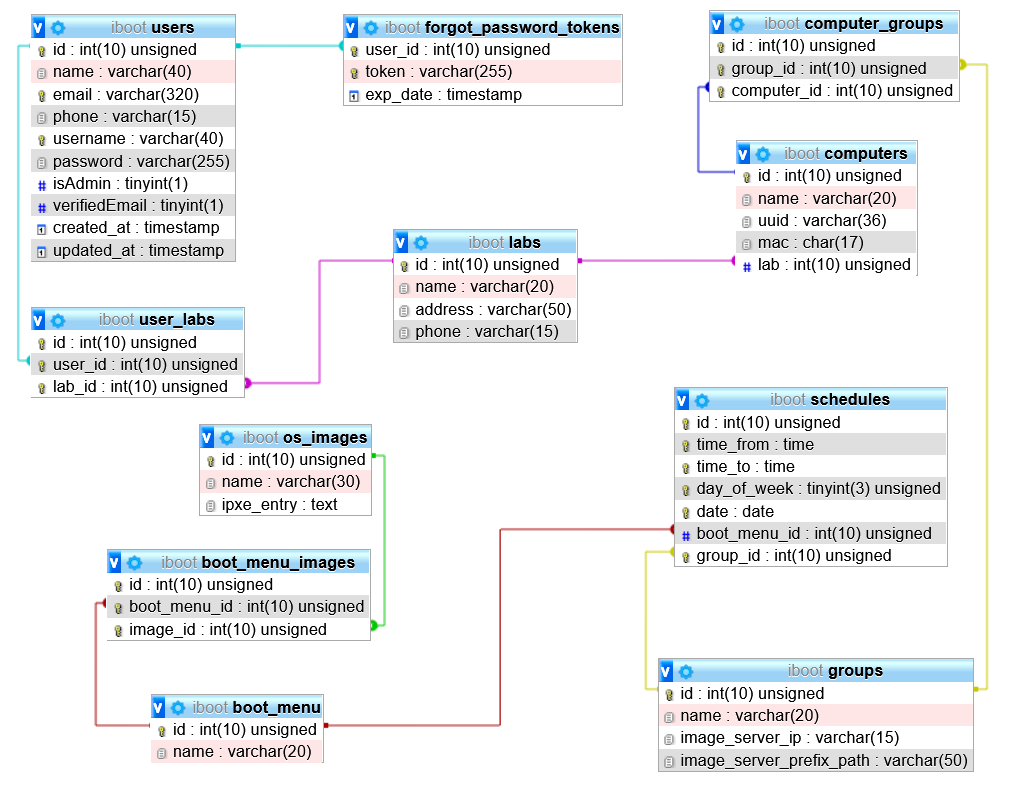
\includegraphics[scale=0.6]{iBoot_database_schema.png}
	\caption{Διάγραμμα Βάσης Δεδομένων iBoot}
	\label{fig:iboot-db}
\end{figure}

Στους πίνακες που ακολουθούν, παρουσιάζονται αναλυτικά οι πίνακες της βάσης δεδομένων του συστήματος, καθώς και τα πεδία τους. Επίσης, ως σχόλιο σε κάθε πεδίο, περιγράφεται η χρησιμότητά του.

\FloatBarrier
%
% Structure: boot_menu
%
\begin{longtable}{|l|c|c|c|l|p{4.5cm}|}
	\caption{Δομή του πίνακα boot\_menu} \label{tab:boot_menu-structure} \\
	\hline \multicolumn{1}{|c|}{\textbf{Στήλη}} & \multicolumn{1}{|c|}{\textbf{Τύπος}} & \multicolumn{1}{|c|}{\textbf{Κενό}} & \multicolumn{1}{|c|}{\textbf{Προεπιλογή}} & \multicolumn{1}{|c|}{\textbf{Σύνδεσμος}} & \multicolumn{1}{|c|}{\textbf{Σχόλιο}} \\ \hline \hline
	\endfirsthead
	\caption{Δομή του πίνακα boot\_menu (συνέχεια)} \\ 
	\hline \multicolumn{1}{|c|}{\textbf{Στήλη}} & \multicolumn{1}{|c|}{\textbf{Τύπος}} & \multicolumn{1}{|c|}{\textbf{Κενό}} & \multicolumn{1}{|c|}{\textbf{Προεπιλογή}} & \multicolumn{1}{|c|}{\textbf{Σύνδεσμος}} & \multicolumn{1}{|c|}{\textbf{Σχόλιο}} \\ \hline \hline \endhead \endfoot 
	\textbf{\textit{id}} & int(10) & Όχι &  &  & Αναγνωριστικό οντότητας \\ \hline 
	name & varchar(20) & Όχι &  &  & Όνομα μενού εκκίνησης \\ \hline 
\end{longtable}

%
% Structure: boot_menu_images
%
\begin{longtable}{|l|c|c|c|l|p{4.5cm}|}
	\caption{Δομή του πίνακα boot\_menu\_images} \label{tab:boot_menu_images-structure} \\
	\hline \multicolumn{1}{|c|}{\textbf{Στήλη}} & \multicolumn{1}{|c|}{\textbf{Τύπος}} & \multicolumn{1}{|c|}{\textbf{Κενό}} & \multicolumn{1}{|c|}{\textbf{Προεπιλογή}} & \multicolumn{1}{|c|}{\textbf{Σύνδεσμος}} & \multicolumn{1}{|c|}{\textbf{Σχόλιο}} \\ \hline \hline
	\endfirsthead
	\caption{Δομή του πίνακα boot\_menu\_images (συνέχεια)} \\ 
	\hline \multicolumn{1}{|c|}{\textbf{Στήλη}} & \multicolumn{1}{|c|}{\textbf{Τύπος}} & \multicolumn{1}{|c|}{\textbf{Κενό}} & \multicolumn{1}{|c|}{\textbf{Προεπιλογή}} & \multicolumn{1}{|c|}{\textbf{Σύνδεσμος}} & \multicolumn{1}{|c|}{\textbf{Σχόλιο}} \\ \hline \hline \endhead \endfoot 
	\textbf{\textit{boot\_menu\_id}} & int(10) & Όχι &  & boot\_menu (id) & Αναγνωριστικό μενού εκκίνησης \\ \hline 
	\textbf{\textit{image\_id}} & int(10) & Όχι &  & os\_images (id) & Αναγνωριστικό εικόνας λειτουργικού συστήματος \\ \hline 
\end{longtable}

%
% Structure: boot_menu_schedules
%
\begin{longtable}{|l|c|c|c|l|p{4.5cm}|}
	\caption{Δομή του πίνακα boot\_menu\_schedules} \label{tab:boot_menu_schedules-structure} \\
	\hline \multicolumn{1}{|c|}{\textbf{Στήλη}} & \multicolumn{1}{|c|}{\textbf{Τύπος}} & \multicolumn{1}{|c|}{\textbf{Κενό}} & \multicolumn{1}{|c|}{\textbf{Προεπιλογή}} & \multicolumn{1}{|c|}{\textbf{Σύνδεσμος}} & \multicolumn{1}{|c|}{\textbf{Σχόλιο}} \\ \hline \hline
	\endfirsthead
	\caption{Δομή του πίνακα boot\_menu\_schedules (συνέχεια)} \\ 
	\hline \multicolumn{1}{|c|}{\textbf{Στήλη}} & \multicolumn{1}{|c|}{\textbf{Τύπος}} & \multicolumn{1}{|c|}{\textbf{Κενό}} & \multicolumn{1}{|c|}{\textbf{Προεπιλογή}} & \multicolumn{1}{|c|}{\textbf{Σύνδεσμος}} & \multicolumn{1}{|c|}{\textbf{Σχόλιο}} \\ \hline \hline \endhead \endfoot 
	\textbf{\textit{id}} & int(10) & Όχι &  &  & Αναγνωριστικό οντότητας \\ \hline 
	time\_from & time & Ναι & ΚΕΝΟ &  & Ώρα έναρξης \\ \hline 
	time\_to & time & Ναι & ΚΕΝΟ &  & 'Ωρα λήξης \\ \hline 
	day\_of\_week & tinyint(3) & Ναι & ΚΕΝΟ &  & Μέρα της εβδομάδας \\ \hline 
	date & date & Ναι & ΚΕΝΟ &  & Ημερομηνία \\ \hline 
	boot\_menu\_id & int(10) & Όχι &  & boot\_menu (id) & Αναγνωριστικό μενού εκκίνησης \\ \hline 
	group\_id & int(10) & Όχι &  & groups (id) & Αναγνωριστικό ομάδας υπολογιστών \\ \hline 
\end{longtable}

%
% Structure: computers
%
\begin{longtable}{|l|c|c|c|l|p{4.5cm}|}
	\caption{Δομή του πίνακα computers} \label{tab:computers-structure} \\
	\hline \multicolumn{1}{|c|}{\textbf{Στήλη}} & \multicolumn{1}{|c|}{\textbf{Τύπος}} & \multicolumn{1}{|c|}{\textbf{Κενό}} & \multicolumn{1}{|c|}{\textbf{Προεπιλογή}} & \multicolumn{1}{|c|}{\textbf{Σύνδεσμος}} & \multicolumn{1}{|c|}{\textbf{Σχόλιο}} \\ \hline \hline
	\endfirsthead
	\caption{Δομή του πίνακα computers (συνέχεια)} \\ 
	\hline \multicolumn{1}{|c|}{\textbf{Στήλη}} & \multicolumn{1}{|c|}{\textbf{Τύπος}} & \multicolumn{1}{|c|}{\textbf{Κενό}} & \multicolumn{1}{|c|}{\textbf{Προεπιλογή}} & \multicolumn{1}{|c|}{\textbf{Σύνδεσμος}} & \multicolumn{1}{|c|}{\textbf{Σχόλιο}} \\ \hline \hline \endhead \endfoot 
	\textbf{\textit{id}} & int(10) & Όχι &  &  & Αναγνωριστικό οντότητας \\ \hline 
	name & varchar(20) & Ναι & ΚΕΝΟ &  & Όνομα υπολογιστή \\ \hline 
	uuid & varchar(36) & Όχι &  &  & Μοναδικό αναγνωριστικό του υπολογιστή, παρεχόμενο από το bios \\ \hline 
	mac & char(17) & Όχι &  &  & Η φυσική διεύθυνση διεπαφής δικτύου του υπολογιστή \\ \hline 
	validated & tinyint(1) & Όχι & 0 &  & Παίρνει τιμή '1' αν ο υπολογιστής έχει γίνει δεκτός στο σύστημα, αλλιώς '0' \\ \hline 
	lab & int(10) & Ναι & ΚΕΝΟ & labs (id) & Αναγνωριστικό εργαστηρίου στο οποίο βρίσκεται ο υπολογιστής \\ \hline 
\end{longtable}

%
% Structure: computer_groups
%
\begin{longtable}{|l|c|c|c|l|p{4.5cm}|}
	\caption{Δομή του πίνακα computer\_groups} \label{tab:computer_groups-structure} \\
	\hline \multicolumn{1}{|c|}{\textbf{Στήλη}} & \multicolumn{1}{|c|}{\textbf{Τύπος}} & \multicolumn{1}{|c|}{\textbf{Κενό}} & \multicolumn{1}{|c|}{\textbf{Προεπιλογή}} & \multicolumn{1}{|c|}{\textbf{Σύνδεσμος}} & \multicolumn{1}{|c|}{\textbf{Σχόλιο}} \\ \hline \hline
	\endfirsthead
	\caption{Δομή του πίνακα computer\_groups (συνέχεια)} \\ 
	\hline \multicolumn{1}{|c|}{\textbf{Στήλη}} & \multicolumn{1}{|c|}{\textbf{Τύπος}} & \multicolumn{1}{|c|}{\textbf{Κενό}} & \multicolumn{1}{|c|}{\textbf{Προεπιλογή}} & \multicolumn{1}{|c|}{\textbf{Σύνδεσμος}} & \multicolumn{1}{|c|}{\textbf{Σχόλιο}} \\ \hline \hline \endhead \endfoot 
	group\_id & int(10) & Όχι &  & groups (id) & Αναγνωριστικό ομάδας υπολογιστών \\ \hline 
	computer\_id & int(10) & Όχι &  & computers (id) & Αναγνωριστικό υπολογιστή \\ \hline 
\end{longtable}

%
% Structure: forgot_password_tokens
%
\begin{longtable}{|l|c|c|c|l|p{4.5cm}|}
	\caption{Δομή του πίνακα forgot\_password\_tokens} \label{tab:forgot_password_tokens-structure} \\
	\hline \multicolumn{1}{|c|}{\textbf{Στήλη}} & \multicolumn{1}{|c|}{\textbf{Τύπος}} & \multicolumn{1}{|c|}{\textbf{Κενό}} & \multicolumn{1}{|c|}{\textbf{Προεπιλογή}} & \multicolumn{1}{|c|}{\textbf{Σύνδεσμος}} & \multicolumn{1}{|c|}{\textbf{Σχόλιο}} \\ \hline \hline
	\endfirsthead
	\caption{Δομή του πίνακα forgot\_password\_tokens (συνέχεια)} \\ 
	\hline \multicolumn{1}{|c|}{\textbf{Στήλη}} & \multicolumn{1}{|c|}{\textbf{Τύπος}} & \multicolumn{1}{|c|}{\textbf{Κενό}} & \multicolumn{1}{|c|}{\textbf{Προεπιλογή}} & \multicolumn{1}{|c|}{\textbf{Σύνδεσμος}} & \multicolumn{1}{|c|}{\textbf{Σχόλιο}} \\ \hline \hline \endhead \endfoot 
	\textbf{\textit{user\_id}} & int(10) & Όχι &  & users (id) & Αναγνωριστικό χρήστη \\ \hline 
	\textbf{token} & varchar(255) & Ναι & ΚΕΝΟ &  & Αλφαριθμητικό αλλαγής κωδικού πρόσβασης \\ \hline 
	exp\_date & timestamp & Ναι & ΚΕΝΟ &  & Ημερομηνία λήξης αλφαριθμητικού \\ \hline 
\end{longtable}

%
% Structure: groups
%
\begin{longtable}{|l|c|c|c|l|p{4.5cm}|}
	\caption{Δομή του πίνακα groups} \label{tab:groups-structure} \\
	\hline \multicolumn{1}{|c|}{\textbf{Στήλη}} & \multicolumn{1}{|c|}{\textbf{Τύπος}} & \multicolumn{1}{|c|}{\textbf{Κενό}} & \multicolumn{1}{|c|}{\textbf{Προεπιλογή}} & \multicolumn{1}{|c|}{\textbf{Σύνδεσμος}} & \multicolumn{1}{|c|}{\textbf{Σχόλιο}} \\ \hline \hline
	\endfirsthead
	\caption{Δομή του πίνακα groups (συνέχεια)} \\ 
	\hline \multicolumn{1}{|c|}{\textbf{Στήλη}} & \multicolumn{1}{|c|}{\textbf{Τύπος}} & \multicolumn{1}{|c|}{\textbf{Κενό}} & \multicolumn{1}{|c|}{\textbf{Προεπιλογή}} & \multicolumn{1}{|c|}{\textbf{Σύνδεσμος}} & \multicolumn{1}{|c|}{\textbf{Σχόλιο}} \\ \hline \hline \endhead \endfoot 
	\textbf{\textit{id}} & int(10) & Όχι &  &  & Αναγνωριστικό οντότητας \\ \hline 
	name & varchar(20) & Όχι &  &  & Όνομα ομάδας \\ \hline 
	image\_server\_ip & varchar(15) & Όχι &  &  & Διεύθυνση server εικόνων \\ \hline 
	image\_server\_prefix\_path & varchar(50) & Όχι &  &  & Πρόθεμα διεύθυνσης εικόνων \\ \hline 
\end{longtable}

%
% Structure: labs
%
\begin{longtable}{|l|c|c|c|l|p{4.5cm}|}
	\caption{Δομή του πίνακα labs} \label{tab:labs-structure} \\
	\hline \multicolumn{1}{|c|}{\textbf{Στήλη}} & \multicolumn{1}{|c|}{\textbf{Τύπος}} & \multicolumn{1}{|c|}{\textbf{Κενό}} & \multicolumn{1}{|c|}{\textbf{Προεπιλογή}} & \multicolumn{1}{|c|}{\textbf{Σύνδεσμος}} & \multicolumn{1}{|c|}{\textbf{Σχόλιο}} \\ \hline \hline
	\endfirsthead
	\caption{Δομή του πίνακα labs (συνέχεια)} \\ 
	\hline \multicolumn{1}{|c|}{\textbf{Στήλη}} & \multicolumn{1}{|c|}{\textbf{Τύπος}} & \multicolumn{1}{|c|}{\textbf{Κενό}} & \multicolumn{1}{|c|}{\textbf{Προεπιλογή}} & \multicolumn{1}{|c|}{\textbf{Σύνδεσμος}} & \multicolumn{1}{|c|}{\textbf{Σχόλιο}} \\ \hline \hline \endhead \endfoot 
	\textbf{\textit{id}} & int(10) & Όχι &  &  & Αναγνωριστικό οντότητας \\ \hline 
	name & varchar(20) & Όχι &  &  & Όνομα εργαστηρίου \\ \hline 
	address & varchar(50) & Ναι & ΚΕΝΟ &  & Διεύθυνση εργαστηρίου \\ \hline 
	phone & varchar(15) & Ναι & ΚΕΝΟ &  & Τηλέφωνο εργαστηρίου \\ \hline 
\end{longtable}

%
% Structure: os_images
%
\begin{longtable}{|l|c|c|c|l|p{4.5cm}|}
	\caption{Δομή του πίνακα os\_images} \label{tab:os_images-structure} \\
	\hline \multicolumn{1}{|c|}{\textbf{Στήλη}} & \multicolumn{1}{|c|}{\textbf{Τύπος}} & \multicolumn{1}{|c|}{\textbf{Κενό}} & \multicolumn{1}{|c|}{\textbf{Προεπιλογή}} & \multicolumn{1}{|c|}{\textbf{Σύνδεσμος}} & \multicolumn{1}{|c|}{\textbf{Σχόλιο}} \\ \hline \hline
	\endfirsthead
	\caption{Δομή του πίνακα os\_images (συνέχεια)} \\ 
	\hline \multicolumn{1}{|c|}{\textbf{Στήλη}} & \multicolumn{1}{|c|}{\textbf{Τύπος}} & \multicolumn{1}{|c|}{\textbf{Κενό}} & \multicolumn{1}{|c|}{\textbf{Προεπιλογή}} & \multicolumn{1}{|c|}{\textbf{Σύνδεσμος}} & \multicolumn{1}{|c|}{\textbf{Σχόλιο}} \\ \hline \hline \endhead \endfoot 
	\textbf{\textit{id}} & int(10) & Όχι &  &  & Αναγνωριστικό οντότητας \\ \hline 
	name & varchar(30) & Όχι &  &  & Το όνομα της εικόνας λειτουργικού συστήματος \\ \hline 
	ipxe\_entry & text & Όχι &  &  & Η ipxe εγγραφή για την εκκίνηση της εικόνας \\ \hline 
\end{longtable}

%
% Structure: users
%
\begin{longtable}{|l|c|c|c|l|p{4.5cm}|}
	\caption{Δομή του πίνακα users} \label{tab:users-structure} \\
	\hline \multicolumn{1}{|c|}{\textbf{Στήλη}} & \multicolumn{1}{|c|}{\textbf{Τύπος}} & \multicolumn{1}{|c|}{\textbf{Κενό}} & \multicolumn{1}{|c|}{\textbf{Προεπιλογή}} & \multicolumn{1}{|c|}{\textbf{Σύνδεσμος}} & \multicolumn{1}{|c|}{\textbf{Σχόλιο}} \\ \hline \hline
	\endfirsthead
	\caption{Δομή του πίνακα users (συνέχεια)} \\ 
	\hline \multicolumn{1}{|c|}{\textbf{Στήλη}} & \multicolumn{1}{|c|}{\textbf{Τύπος}} & \multicolumn{1}{|c|}{\textbf{Κενό}} & \multicolumn{1}{|c|}{\textbf{Προεπιλογή}} & \multicolumn{1}{|c|}{\textbf{Σύνδεσμος}} & \multicolumn{1}{|c|}{\textbf{Σχόλιο}} \\ \hline \hline \endhead \endfoot 
	\textbf{\textit{id}} & int(10) & Όχι &  &  & Αναγνωριστικό οντότητας \\ \hline 
	name & varchar(40) & Όχι &  &  & Ονοματεπώνυμο \\ \hline 
	\textbf{email} & varchar(320) & Όχι &  &  & Διεύθυνση email\\ \hline 
	phone & varchar(15) & Ναι & ΚΕΝΟ &  & Αριθμός τηλεφώνου \\ \hline 
	\textbf{username} & varchar(40) & Όχι &  &  & Όνομα χρήστη \\ \hline 
	password & varchar(255) & Όχι &  &  & Κωδικός πρόσβασης \\ \hline 
	admin & tinyint(1) & Όχι & 0 &  & Παίρνει τιμή '1' αν ο χρήστης είναι γενικός διαχειριστής, αλλιώς '0' \\ \hline 
	accepted & tinyint(1) & Όχι & 0 &  & Παίρνει τιμή '1' αν ο χρήστης έχει γίνει δεκτός στο σύστημα, αλλιώς '0' \\ \hline 
	verifiedEmail & tinyint(1) & Όχι & 0 &  & Παίρνει τιμή '1' αν ο χρήστης έχει επιβεβαιώσει τη διεύθυνση email του, αλλιώς '0' \\ \hline 
	created\_at & timestamp & Ναι & ΚΕΝΟ &  & Ημερομηνία δημιουργίας του χρήστη \\ \hline 
	updated\_at & timestamp & Ναι & ΚΕΝΟ &  & Ημερομηνία ενημέρωσης του χρήστη \\ \hline 
\end{longtable}

%
% Structure: user_labs
%
\begin{longtable}{|l|c|c|c|l|p{4.5cm}|}
	\caption{Δομή του πίνακα user\_labs} \label{tab:user_labs-structure} \\
	\hline \multicolumn{1}{|c|}{\textbf{Στήλη}} & \multicolumn{1}{|c|}{\textbf{Τύπος}} & \multicolumn{1}{|c|}{\textbf{Κενό}} & \multicolumn{1}{|c|}{\textbf{Προεπιλογή}} & \multicolumn{1}{|c|}{\textbf{Σύνδεσμος}} & \multicolumn{1}{|c|}{\textbf{Σχόλιο}} \\ \hline \hline
	\endfirsthead
	\caption{Δομή του πίνακα user\_labs (συνέχεια)} \\ 
	\hline \multicolumn{1}{|c|}{\textbf{Στήλη}} & \multicolumn{1}{|c|}{\textbf{Τύπος}} & \multicolumn{1}{|c|}{\textbf{Κενό}} & \multicolumn{1}{|c|}{\textbf{Προεπιλογή}} & \multicolumn{1}{|c|}{\textbf{Σύνδεσμος}} & \multicolumn{1}{|c|}{\textbf{Σχόλιο}} \\ \hline \hline \endhead \endfoot 
	\textbf{\textit{user\_id}} & int(10) & Όχι &  & users (id) & Αναγνωριστικό χρήστη \\ \hline 
	\textbf{\textit{lab\_id}} & int(10) & Όχι &  & labs (id) & Αναγνωριστικό εργαστηρίου \\ \hline 
\end{longtable}

\FloatBarrier

\section{Επεξήγηση Αρχείων}

\section{Ασφάλεια Συστήματος}

\section{Σύνοψη Κεφαλαίου 3}
Η δομή και η οργάνωση του εφαρμοζόμενου πληροφοριακού συστήματος είναι τα θέματα που καλύπτονται στην ανάλυση του κεφαλαίου 3. Στην αρχή, περιγράφηκαν οι στόχοι, οι λειτουργικές απαιτήσεις και οι περιπτώσεις χρήσης. Επιπλέον, εξετάστηκαν το σχεσιακό διάγραμμα και τα μοντέλα των πινάκων της βάσης δεδομένων και δόθηκε μια λεπτομερής εξήγηση του σχεδιασμού της βάσης δεδομένων. Στη συνέχεια, εξηγήθηκαν διεξοδικά τόσο το front-end όσο και το back-end της δομής του πληροφοριακού συστήματος. τα αρχεία προγραμμάτων υπολογιστών που εκτελούν τις πρωταρχικές λειτουργίες του συστήματος. Προκειμένου να διασφαλιστεί η ασφάλεια κατά τη χρήση της διαδικτυακής εφαρμογής, παρέχεται επεξήγηση των πρωτοκόλλων και των προσεγγίσεων ασφαλείας.

Στο κεφάλαιο 4, αναλύονται τα βήματα που ο χρήστης πρέπει να ακολουθήσει για να χρησιμοποιήσει την εφαρμογή.
